\documentclass[12pt] {article}
\usepackage{times}
\usepackage[margin=0.6in,bottom=1in,top=0.5in]{geometry}

\usepackage{hhline}
\usepackage{subfig}
\usepackage{graphicx}
\usepackage{amsmath}




\begin{document}

\title{Final Project}
\author{Yuxin Chen and Ruolan Zeng}
\date{March 22nd, 2018}
\maketitle
%============Table========
%\begin{figure}[tbh]
% \centering    
%\begin{tabular}{ |p{4cm}|| p{2cm}|p{2cm}|p{2cm}|p{2cm}|}
% \hline
% & Processor 1 &  Processor 2  & Processor 3 & Processor 4\\ \hhline{|=|=|=|=|=|}
% \hline
% Performance          &$1.08$        &$1.425$       &\textbf{1.52}  &   \\
% \hline
%\end{tabular} 
%\caption{Metric table for the four processors}
%   \label{tab:metric}
%\end{figure} 
%============Figure========
%\begin{figure}[!tbh]
%\centering        
%   \subfloat {\includegraphics[width=0.65\textwidth]{fig2_4.png}}
%   \caption{ }
%   \label{fig:fig}
%\end{figure}

\section*{Algorithm Details:}
Generally, there are two approach to do graph coloring: 1) independent set (IDS) based 2) greedy algorithm based. In our work, we chose to use independent set based algorithm. %Basically we generate a random number for each node, then a node an be added to the current independent set only if it has the maximum random number among its neighbors. This method ensures every node within the same independent set to be colored , they are not connected. Next iteration we find the maximum vertex on nodes left (exclude nodes which are in the independent sets) and form a new indepedent set. The algorithm continues untill all the nodes belong to independent sets.
The IDS-based algorithm first assigns random number for each node in the input graph. Then the algorithm proceeds by adding the nodes with maximum random number among their neighbor (nodes they are connected to) to an independent set. Nodes in an independent set are colored with the same colors and deleted from the graph. The process continues between two phases; finding IDS and coloring the IDS and deleting it from the graph until all nodes are colored. 

\subsection*{An naive implementation}
An naive implementation: 
%\begin{figure}[!tbh]
%\centering        
%   \subfloat {\includegraphics[width=0.5\textwidth]{naive.jpg}} 
%   \caption{Overview of IDS based graph coloring.}
%   \label{fig:fig1}
%\end{figure}

Each iteration, each thread access one node, it will see first if its InIDS value (is in the independent set?) is 1, if yes, it exits, if no, it needs to see its neighbor's InIDS value and only compares the node's random number with its neighbor's whose InIDS value is 0. If it is the maximum among its neighbors, it first writes itself into independent set IDS0 (or IDS1, IDS2, dependent on the iteration), and set the node's InIDS value to 1. Then it goes to next iteration. 

So if at this iteration, a node is not included into an independent set, next iteration, it still needs to compare with its live neighbors (dead if some node are included in an independent set). This node will keep using the same neighbor list until it is added to an independent set. There is potential two improvement for this naive implementation: 1) since some thread will access node that are in independent sets, then exits immediately. Since threads are executed in warps, if half of the threads in a warp exit immediately, then we wasting computing cycles and under utilize the hardware. 2) data reuse. Now all the memory access goes through global memory. We should think about using shared memory.

Now just think about how to use shared memory, if we distributed nodes to different blocks, each node can load its neighbor list into shared memory and reuse it until it is added to an independent set. However, each iteration, the node also needs to know its neighbor's status (if added to IDS). If its neighbor belongs to other block, it is hard to keep data coherency among blocks. 

\subsection*{Communication free graph coloring}
We propose this communication free (CF) graph coloring approach:

%\begin{figure}[!tbh]
%\centering        
%   \subfloat {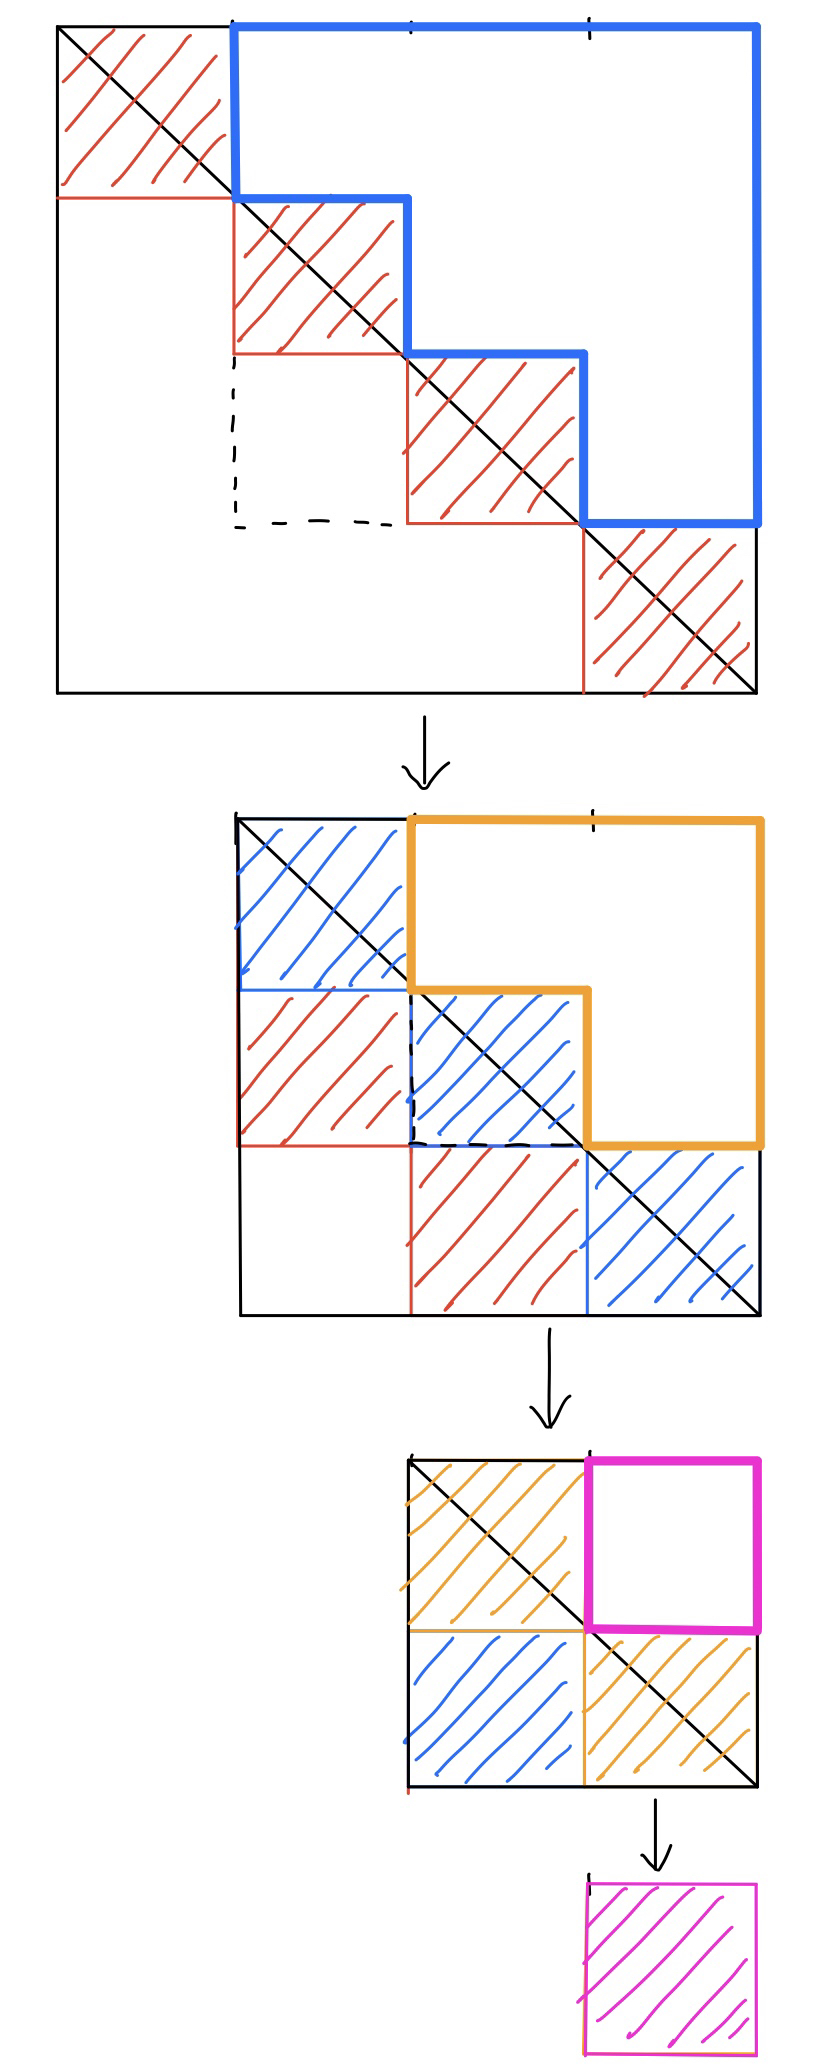
\includegraphics[width=0.5\textwidth]{comfree.jpg}}
%   \caption{Overview of communication free graph coloring.}
%   \label{fig:fig2}
%\end{figure} 

When we run local graph coloring, we use the algorithm we describe above and ignoring the node's neighbors that are on other blocks, i.e., we don't examine the neighbor which belongs to other blocks. After each block finishes local graph coloring, the conflict can only happen between nodes that belongs to different blocks. Then we extract those nodes only and form a new conflict graph and resolve those conflict by assigning new colors to subset of the conflicting nodes (and leave the others as they are). We are expecting, in practices, the conflict graph would be small %and the number of colors used in local graph coloring will not bad. 
Because we run local graph coloring in shared memory, it should be fast. 

\section*{Implementation:}

\subsection*{Local graph coloring}
The local coloring kernel divides the graph into number of blocks. Each block will only read the information of the nodes assigned to it i.e., subset of a modified CSR of the adjacency matrix. At the end of this kernel, all nodes assigned to a block will have correct colors (no conflict). However, conflict may occur between nodes assigned to different blocks. We aim to make this phase fast and, secondary, gives decent amount of colors. For that, instead of create and moving an array of random numbers, we use the column ID array as the random number. For example if node 0 and 10 are connected and in the same block, we pick 10 to be in the independent set. Since we need to check if a node is in the independent set and its connectivity frequently, we use shared memory  to store this data specially that the block size is small (to make it fast) and so that data fits in the shared memory. Also, the colors are written into the shared memory before writing it to the global memory. We made sure that all memory memory write and read are coalesced. 
\subsection*{Conflict resolve}
%After the steps above, we have the conflict graph which is a format of CSR grouped by color. 
After the local coloring, we prepare the conflict graph in parallel. This graph is in CSR format that encapsulates the information of a matrix with columns as the nodes and rows as the assigned color. In other words, it is a histogram of the assigned colors. We process each color in sequence. We can definitely process all the color generated in previous step in parallel and each block will get one color, so there is a load balancing problem. %and we don't have time to do that. 

Given an array of conflict nodes of same color, we resolve the conflict by finding the neighbors of each node who has the same color and comparing the node ID with its conflict neighbor's ID, the one with lower ID will not change color, the one with higher ID will be assigned a new color. 

Here we give an example for nodes [1,2,3,4] that are conflict nodes whose color is red and node 1 connects to node 3, node 2 connects to node 4. Then we run the algorithm, node 1 will find node 3 is its neighbor, but node 3's ID is higher, then, node 1 will not change its color. Node 3 will find node 1 is its neighbor, and node 1's ID is lower than its ID, then, node 3 will change its color to a new color purple. Some thing for node 2 and node 4, node 2 will not change its color and node 4 will change its color to new color purple. Then we need to review those nodes which ared assigned new color again to ensure they are not conflict to each other. Then we find out node 3's neighbor, and find out node 3 doesn't have conflict neighbors, and for node 4, find out node 4 doesn't have conflict neighbors. Then the conflict nodes originally in color red now are resolved. If node 3 and node 4 are connected, then, we will find out node 3 won't change color since it has lower ID and node 4 will be assigned a new color yellow. We will need to review all the changed color nodes again which is node 4 and find out node 4 doesn't have conflict and all the conflict resolved. 

We do the above process for each color sequentially. After that, we can resolve all the conflict. 

There are some implementation optimization:
\begin{itemize}
\item When we get a node and need to find out its neighbor, since the neighbor whose ID is higher than the node, we won't change the node's color. We should not examine its neighbor whose ID is higher. We can achieve this by just using the lower triangle of the graph adjacency matrix. 

\item What we start with is an array of conflict nodes.

%\begin{figure}[!tbh]
%\centering        
%   \subfloat {\includegraphics[width=0.5\textwidth]{confre.jpg}}
%   \caption{Data structure of CF graph coloring.}
%   \label{fig:fig3}
%\end{figure} 

We want to get each node's neighbor list to tell if we need change this nodes' color. However if we map each thread to a node in the node array and read its neighbor list and see if the node need change color, we will have very unbalanced work load for each thread, since the neighbor list for each node can vary a lot, then we are wasting computing cycle waiting for the thread who works on the longest neighbor list. We would prefer each thread work on each neighbor of each node. To have enough information to achieve this mapping, we need to do extra work:

%\begin{figure}[!tbh]
%\centering        
%   \subfloat {\includegraphics[width=0.5\textwidth]{scanlbswir.jpg}}
%   \caption{Details of CF load balancing.}
%   \label{fig:fig4}
%\end{figure} 

First we ask each thread to load a neighbor of a node and save it in register. To do this, each thread need to know which node's neighbor list, and the position of that neighbor in that neighbor list. To compute which node's neighbor list each thread need to access, we fist compute neighLen array by each thread get the neighbor list's length of each node, then we do scan on neighLen and compute load balancing search on the scan result. To compute the position each thread should access in assigned neighbor list, we compute the work item rank ($wir$) array by computing $lbs[i]=i-scan[lbs[i]]$. After this, each thread can access each neighbor just using $tr\_col\_id[tr\_offset[nodes[lbs[i]]] + wir[i]]$, where $tr\_col\_id$ is the CSR column ID array for the conflict graph and $tr\_offset$ is the CSR row offset array for the conflict graph. Now we can examine the neighbor's color and produce a predicate array of if change color. Using this changeColor array, we can assign new color to nodes who need change color and do scan on changeColor, we can compact those nodes who need change color into a new array. Then go back to the top of the loop until there is no node who need to change color.

\end{itemize}

%\section{Other approach}
%Another good approach is to distribute nodes to different blocks and generate a random number each iteration and synchronize all the blocks using cooperative group in CUDA 9 or above. Then we can keep the neighbor list in the share memory all the time. One consideration is it is better for each node have a different random number otherwise it will increase the number of iteration to finish coloring. If we set the random number range large enough, the probability to get same random number for different nodes is very low.

\section*{Numerical Experiments:}
Here we show some results of our implementation. Table ~\ref{tab:results} shows the results and comparison against greedy algorithm. We found that even though in the local coloring using the column id as the random number would decrease the amount of memory transfer, but the color would depend on the listing of nodes which is very likely to be not random. This could be one reason why we get larger number of colors. Another reason, is the blocking size given to the local coloring kernel which need fine tuning in order to reach an optimal number of color that our implementation can produce. 


\begin{figure}[tbh]
 \centering    
\begin{tabular}{ |p{4cm}||p{3cm}|| p{4cm}|p{4cm}|}
 \hline
   & $\#$Vertices & Our Implementation &  Greedy \\ 
     
     \hhline{|=||=||=|=|}
 \hline
 le450\_5d.col &450       & 58  &18 \\
 \hline
 myciel4.col &  23       & 8  &5 \\
 \hline
  planar16.col &16        & 7  &5 \\
 \hline
  planar36864.col & 36864     & 19  &7 \\
 \hline
   planar40.col &  40      & 9  & 5\\
 \hline
   planar43264.col & 43264     &  20 & 7\\
 \hline
 
 
\end{tabular} 
\caption{Results and comparsion of our implementation against CPU greedy algorithm.}
   \label{tab:results}
\end{figure} 

\begin{figure}[tbh]
 \centering    
\begin{tabular}{ |p{4cm}||p{3cm}|| p{4cm}|p{4cm}|}
 \hline
   & $\#$Naive & Three Kernels &  Load Balancing Search \\ 
     
     \hhline{|=||=||=|=|}
 \hline
 le450\_5d.col &450       & 58  &18 \\
 \hline
 myciel4.col &  23       & 8  &5 \\
 \hline
  planar16.col &16        & 7  &5 \\
 \hline
  planar36864.col & 36864     & 19  &7 \\
 \hline
   planar40.col &  40      & 9  & 5\\
 \hline
   planar43264.col & 43264     &  20 & 7\\
 \hline
   qg.order100.col &
 
 
\end{tabular} 
\caption{Results and comparsion of our implementation against CPU greedy algorithm.}
   \label{tab:results}
\end{figure} 

Because of the algorithm, the test run on qg.order100.col will use more than 256 colors. However, we use array of unsigned char to record the colors. So our algorihtm failed on this test case.


\end{document}
